%& --shell-escape
%& --shell-escape
\documentclass[%
12pt%
%,draft
]%
{book} %Klasse

\usepackage{etex}
\usepackage{hyperref}

\usepackage{setspace}
\usepackage{xspace}
\usepackage{float}
\usepackage{framed}

%\usepackage[margin=12pt, font=large,format=plain,labelfont=small,up]{caption}
\usepackage[margin=12pt, font=footnotesize,format=plain,labelfont=bf,up]{caption}
%\usepackage[font=footnotesize]{caption}
\usepackage{color}

%\usepackage[right=25mm, left=25mm, bottom=30mm, top=25mm]{geometry}
\usepackage{geometry}

\usepackage{supertabular}
\usepackage{rotating} 
\usepackage{multirow}

\usepackage{enumerate}

\usepackage{pdfpages}
\usepackage[authoryear]{natbib}

%% new comands
\newcommand{\cglut}{\textit{C.\,glu\-ta\-mi\-cum}\xspace}
\newcommand{\dfifo}{\textit{C.\,glu\-ta\-mi\-cum}\,$\Delta$F$_1$F$_0$\xspace}
\newcommand{\ilva}{\textit{C.\,glu\-ta\-mi\-cum}\,\textit{$\Delta$ilvA}\xspace}
\newcommand{\glgc}{\textit{C.\,glu\-ta\-mi\-cum}\,\textit{$\Delta$ilvA$\Delta$glgC}\xspace}
\newcommand{\mfa}{$^{13}$C-MFA\xspace}
\newcommand{\glcI}{$^{13}C_1$-glucose\xspace}
\newcommand{\tr}{\textcolor{red}}
%\newcommand{\dummy}{\includegraphics[width=0.2\textwidth]{tikz/LegoDummy.jpg}}
\newcommand{\dummy}{\includegraphics[width=0.2\textwidth]{tikz/dummy.jpg}}
\newcommand{\omix}{\texttt{Omix}{\small\textsuperscript{\textregistered}}\xspace}
%\newcommand{\omix}{\texttt{Omix}\textsuperscript{\small \textregistered}\xspace}
\newcommand{\xflux}{\texttt{13CFLUX2}\xspace}
\newcommand{\atpase}{F$_1$F$_0$-ATP synthase\xspace}

\usepackage[sumlimits,intlimits,namelimits]{amsmath}

\usepackage{listings}
%\usepackage{xfrac}

\usepackage{rotating}
\usepackage{longtable, lscape}
\usepackage{caption}
% ================================================================================
%% Tikz von Samuel

\usepackage{tikz}
\usepackage{pgfplots}
\usepackage{pgfplotstable} % csv einlesen und daraus tabellen und plots...
\usepackage{booktabs} % Fuer rules in pgfplotstable-preset
\usepackage{ifthen}
\usepackage{xstring}
\usepackage{filemod}

\usetikzlibrary{external}
\usetikzlibrary{arrows,shapes,intersections}
\usetikzlibrary{plotmarks}
\usetikzlibrary{calc}

\tikzsetexternalprefix{tikzcache/}
\tikzset{/tikz/external/only named=true}
\tikzexternalize

\pgfrealjobname{Hauptdokument} % <-- NOTE: this needs to be the real document's basename // Hauptdokument!!!

\pgfplotsset{compat=newest}

\newcommand\parseFilenameSave[2]{%
	\noexpandarg
	\StrCount{#1}{/}[\posOfLastDelimiter]%
	\StrBehind[\posOfLastDelimiter]{#1}{/}[#2]
}

\newcommand{\inputTikZ}[1]{%
  \parseFilenameSave{#1}{\tempFigureNameExternal}%
  \tikzsetnextfilename{\tempFigureNameExternal -external}%
  \filemodCmp{#1.tikz}{tikzcache/\tempFigureNameExternal -external.log}%
  {\tikzset{external/remake next}\input{#1.tikz}}{\input{#1.tikz}}%
%  \input{#1.tikz}%
}

\usepackage{subcaption}

% ================================================================================

\usepackage{xcolor}
%\newcommand{\MyColor}{colormap={FZJblue}{rgb255(0cm)=(41,189,255); rgb255(1cm)=(0,91,130)}}
%\pgfplotsset{colormap={FZJblue}{rgb255(0cm)=(41,189,255); rgb255(1cm)=(0,91,130)}}
\definecolor{RED}{rgb}{1,0,0}
% defining custom colors
%\definecolor{DarkRed}{rgb}{0.8471,0.1608,0}
%\definecolor{EOrange}{rgb}{1,0.75,0}
%\definecolor{FZJdark}{rgb}{0,0.3569,0.5098}
%\definecolor{FZJslight}{rgb}{0.1608,0.7412,1}
%\definecolor{MyGreen}{rgb}{0,0.6902,0.3137}

%% ROoF PaperHeader
\usepackage{amsmath,amssymb,mathtools} %!!!

\usepackage[english]{babel} %!!!
\usepackage{verbatim} %!!!

%% Load packages
%\usepackage{cite} % Make references as [1-4], not [1,2,3,4]
%\usepackage{url}  % Formatting web addresses  
%\usepackage{ifthen}  % Conditional 
\usepackage{multicol}   %Columns
%\usepackage[utf8]{inputenc} %unicode support
%\urlstyle{rm}

%%% ============================================================================

\newcommand{\mat}[1]{\ensuremath{{\bf #1}}}
\DeclarePairedDelimiter\abs{\lvert}{\rvert}
\DeclarePairedDelimiter\norm{\lVert}{\rVert}
\newcommand{\prozent}[1]{\ensuremath{#1~\%}}
\newcommand{\mean}[1]{\ensuremath{\mu\left(#1\right)}}
\newcommand{\stddev}[1]{\ensuremath{\sigma\left(#1\right)}}

\newcommand{\TruncNormalDist}{\ensuremath{\mathcal{N}_{0, \delta, [- 2\delta, + 2\delta]}}}
\newcommand{\NormalDist}{\ensuremath{\mathcal{N}_{0, \delta}}}
\newcommand{\UniformDist}{\ensuremath{\mathcal{U}_{[-2\delta, \; 2\delta]}}}

\DeclareMathOperator{\rang}{rang}
\DeclareMathOperator{\conv}{conv}
\DeclareMathOperator{\interior}{int}
\DeclareMathOperator{\Var}{Var}
\DeclareMathOperator{\expect}{\mathbb{E}}
\DeclareMathOperator*{\argmax}{arg\,max}

\renewcommand{\vec}[1]{\ensuremath{\boldsymbol{#1}}}

\newcommand{\BIGOP}[1]{\mathop{\mathchoice%
{\raise-0.22em\hbox{\huge $#1$}}%
{\raise-0.05em\hbox{\Large $#1$}}{\hbox{\large $#1$}}{#1}}}
\newcommand{\cart}{\BIGOP{\times}}

\newcommand{\slfrac}[2]{\left.#1\middle/#2\right.}

\newcommand{\matrixLineSpacing}{1.25}

\makeatletter
\renewcommand*\env@matrix[1][r]{\hskip -\arraycolsep
  \let\@ifnextchar\new@ifnextchar
  \array{*\c@MaxMatrixCols #1}}
\makeatother

\makeatletter
\renewcommand*\env@matrix[1][*\c@MaxMatrixCols c]{%
  \hskip -\arraycolsep
  \let\@ifnextchar\new@ifnextchar
  \array{#1}}
\makeatother


\makeatletter
\renewcommand*\env@matrix[1][c]{\hskip -\arraycolsep
  \let\@ifnextchar\new@ifnextchar
  \array{*\c@MaxMatrixCols #1}}
\makeatother

\usepackage{textcomp}
%\textperthousand 	Promille 	textcomp
%\permil 	Promille 	wasysym 

%\tiny
%\scriptsize
%\footnotesize
%\small
%\normalsize
% \large  
%\Large  
%\LARGE
%\huge
%\Huge 


\begin{document}
\pagestyle{empty}

\section*{FBA}
\begin{align}\label{eq: SteadyState}
	\frac{d\vec{c}}{dt} = \vec{0} \Rightarrow  \mat{S} \cdot \vec{v} = \vec{0}.
\end{align}

\begin{align}\label{eq:FluxLimits}
	\vec{\ell} \leq \vec{v} \leq \vec{u}.
\end{align}

\begin{align}\label{eq:AdditionalInequalityConstraints}
	\mat{\tilde{C}} \cdot \vec{v} \leq \vec{\tilde{b}}.
\end{align}

\begin{align}\label{eq:constraints}\renewcommand*{\arraystretch}{\matrixLineSpacing}
	\mat{C} \vec{v} = \begin{pmatrix}[r]
		\mat{\tilde{C}} \\ 
		\mat{I_n} \\
		-\mat{I_n}
	\end{pmatrix} \vec{v} \leq \begin{pmatrix}[r] \vec{\tilde{b}} \\ \vec{u} \\ -\vec{\ell} \end{pmatrix} = \vec{b},
\end{align}
 

\begin{align}\label{eq:objective}
Z(\vec{v}) = \vec{f}^T \vec{v}.
\end{align}

Summarizing,  the following FBA problem is solved using LP:
\begin{align}\label{eq:FBALP}
	\begin{array}{rl}
		\max_{\vec{v}} & \vec{f}^T \vec{v} \\
		\text{s.t.}& \mat{S} \vec{v} = \vec{0} \\
		& \mat{C} \vec{v} \leq \vec{b}.
	\end{array}
\end{align}


\section*{Example Network}
The stoichiometric matrix of the toy network is given as: 

\begin{align}\label{eq:stoichMatrixNw}
\mat{S} = \bordermatrix{~ & v_1 & v_2  & v_3  & v_4  & v_5  & v_6 \cr
A& 1 & 1 & -2 & 0 & 1 & 0 \cr
B& 1 & -1 & 0 & 1 & 0 & 0 \cr
C& 0 & 0 & 1 & -2 & 0 & -1.77 \cr
D& 0 & -1 & 0 & 1 & -1 & 1.38 \cr}
\end{align}

The example network  has two degrees of freedom. Hence the choice of two free fluxes (e.g.\@ $v_1$ and $v_6$) defines all other fluxes and the following equation holds: 

$v_2 = 2 \cdot v_1 + (1.38 - 1.77) \cdot v_6$

$v_3 = (2 \cdot 1.38 - 1.77) \cdot v_6 + 2\cdot v_1$

$v_4 = v_1 + (1.38 - 1.77) \cdot v_6$

$v_5 = 1.38 \cdot v_6 - v_1$

 The reaction rates of the example network (Figure\,\ref{fig: toyNw}) are bounded as follows:
\begin{align}\label{eq:fluxBoundsNw}
	\begin{array}{rl}
& \begin{matrix}
 0  \le v_1,v_5  \le 10 \\
 -10 \le v_2,v_3,v_4 \le 10 \\
0  \le v_6  \le 20
\end{matrix} 
	\end{array}
\end{align}

The feasible flux space is visualized in Figure\,\ref{fig: feasibleSpace}. 

\begin{figure}[htb]
\centering
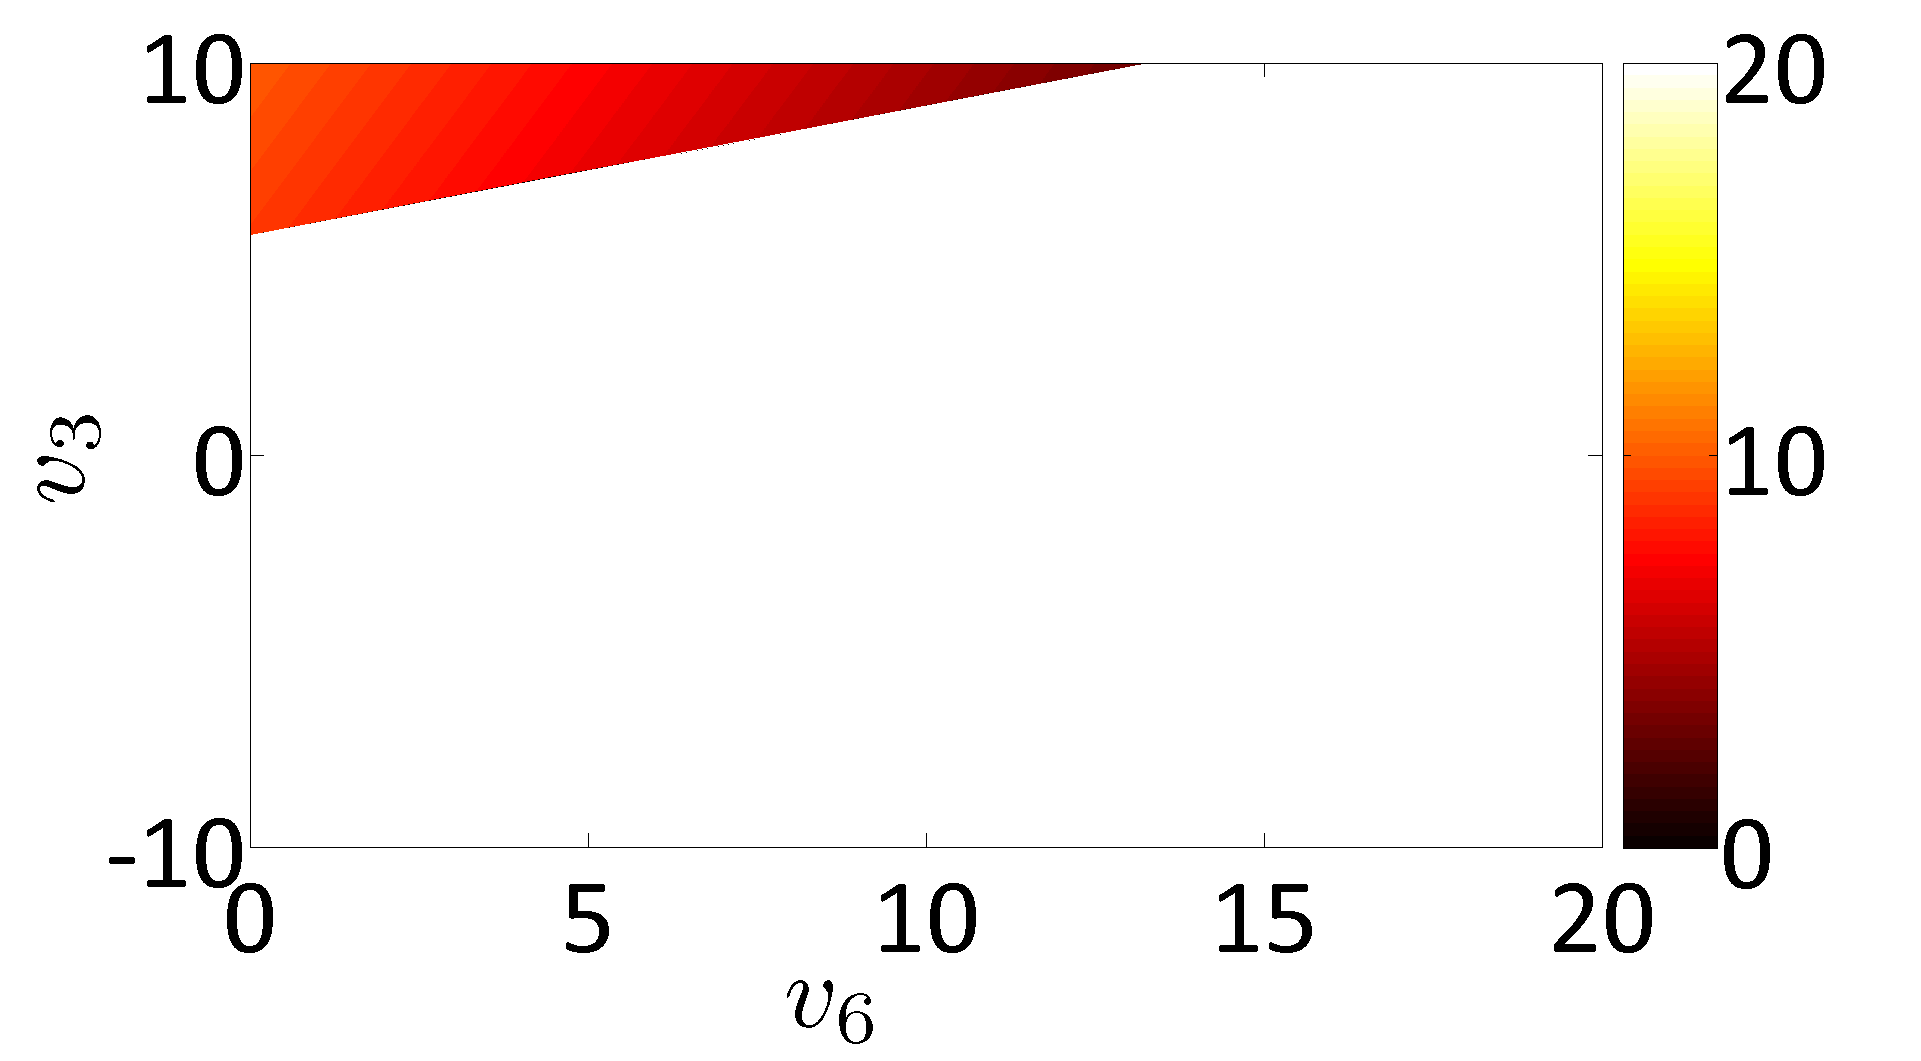
\includegraphics[width=0.75\textwidth]{SolutionSpaceToyNw.png}
\caption{Intersection of a hyperplane with the flux solution space (the uptake is fixed: $v_1=8.4$). On the axes the flux range for $v_6$ (x-axis) and $v_3$ (y-axis) are shown. Due to the interdependencies between the fluxes the flux polytope is restricted. Thus, the remaining feasible solution space is represented by the colored area. When optimizing reaction $v_6$ (x-axis), the optimal value can be read off.}
\end{figure}


For the example network the criterion of optimality might be the maximization of the flux through reaction $v_6$. Metabolite D represents an artificial biomass metabolite. 

The FBA problem is then given by:
\begin{align}\label{eq:FBAtoyNw}
	\begin{array}{r l l}
		\max_{\vec{v}} 	& Z(\vec{v}) &= \vec{v}_6\\
		\text{s.t.}	  	& \mat{S} \vec{v} &=  \vec{0} \\
				  	&  v_{1,5}  & \in[0,10] \\
					&  v_{2,3,4} & \in [-10,10] \\
					&  v_6  & \in [0, 20] \\
	\end{array}
\end{align}

Solving the LP problem yields a maximal flux of $\frac{40}{3}$ through reaction $v_6$. The optimal flux solution (given in arbitrary units) is:
\begin{align}\label{eq:optToyNw}
 \vec{v} = \frac{1}{15}(126,24,150,-102,150,200)^T
\end{align}
Comparing the optimal flux distribution with the flux bounds reveals that a further increase of the objective is hampered by $v_3$ or $v_5$, because both reactions have the maximal allowed flux. 

\end{document}